% Options for packages loaded elsewhere
\PassOptionsToPackage{unicode}{hyperref}
\PassOptionsToPackage{hyphens}{url}
%
\documentclass[
  9pt,
  ignorenonframetext,
  aspectratio=169,
]{beamer}
\usepackage{pgfpages}
\setbeamertemplate{caption}[numbered]
\setbeamertemplate{caption label separator}{: }
\setbeamercolor{caption name}{fg=normal text.fg}
\beamertemplatenavigationsymbolsframe
% Prevent slide breaks in the middle of a paragraph
\widowpenalties 1 10000
\raggedbottom
\setbeamertemplate{part page}{
  \centering
  \begin{beamercolorbox}[sep=16pt,center]{part title}
    \usebeamerfont{part title}\insertpart\par
  \end{beamercolorbox}
}
\setbeamertemplate{section page}{
  \centering
  \begin{beamercolorbox}[sep=12pt,center]{part title}
    \usebeamerfont{section title}\insertsection\par
  \end{beamercolorbox}
}
\setbeamertemplate{subsection page}{
  \centering
  \begin{beamercolorbox}[sep=8pt,center]{part title}
    \usebeamerfont{subsection title}\insertsubsection\par
  \end{beamercolorbox}
}
\AtBeginPart{
  \frame{\partpage}
}
\AtBeginSection{
  \ifbibliography
  \else
    \frame{\sectionpage}
  \fi
}
\AtBeginSubsection{
  \frame{\subsectionpage}
}
\usepackage[]{roboto}
\usepackage{amssymb,amsmath}
\usepackage{ifxetex,ifluatex}
\ifnum 0\ifxetex 1\fi\ifluatex 1\fi=0 % if pdftex
  \usepackage[T1]{fontenc}
  \usepackage[utf8]{inputenc}
  \usepackage{textcomp} % provide euro and other symbols
\else % if luatex or xetex
  \usepackage{unicode-math}
  \defaultfontfeatures{Scale=MatchLowercase}
  \defaultfontfeatures[\rmfamily]{Ligatures=TeX,Scale=1}
\fi
\usetheme[]{Dresden}
\usecolortheme{beaver}
% Use upquote if available, for straight quotes in verbatim environments
\IfFileExists{upquote.sty}{\usepackage{upquote}}{}
\IfFileExists{microtype.sty}{% use microtype if available
  \usepackage[]{microtype}
  \UseMicrotypeSet[protrusion]{basicmath} % disable protrusion for tt fonts
}{}
\makeatletter
\@ifundefined{KOMAClassName}{% if non-KOMA class
  \IfFileExists{parskip.sty}{%
    \usepackage{parskip}
  }{% else
    \setlength{\parindent}{0pt}
    \setlength{\parskip}{6pt plus 2pt minus 1pt}}
}{% if KOMA class
  \KOMAoptions{parskip=half}}
\makeatother
\usepackage{xcolor}
\IfFileExists{xurl.sty}{\usepackage{xurl}}{} % add URL line breaks if available
\IfFileExists{bookmark.sty}{\usepackage{bookmark}}{\usepackage{hyperref}}
\hypersetup{
  pdfauthor={Luis Kress, Johannes Hausmann},
  hidelinks,
  pdfcreator={LaTeX via pandoc}}
\urlstyle{same} % disable monospaced font for URLs
\newif\ifbibliography
\usepackage{graphicx}
\makeatletter
\def\maxwidth{\ifdim\Gin@nat@width>\linewidth\linewidth\else\Gin@nat@width\fi}
\def\maxheight{\ifdim\Gin@nat@height>\textheight\textheight\else\Gin@nat@height\fi}
\makeatother
% Scale images if necessary, so that they will not overflow the page
% margins by default, and it is still possible to overwrite the defaults
% using explicit options in \includegraphics[width, height, ...]{}
\setkeys{Gin}{width=\maxwidth,height=\maxheight,keepaspectratio}
% Set default figure placement to htbp
\makeatletter
\def\fps@figure{htbp}
\makeatother
\setlength{\emergencystretch}{3em} % prevent overfull lines
\providecommand{\tightlist}{%
  \setlength{\itemsep}{0pt}\setlength{\parskip}{0pt}}
\setcounter{secnumdepth}{5}
\pagestyle{plain}
\newlength{\cslhangindent}
\setlength{\cslhangindent}{1.5em}
\newenvironment{cslreferences}%
  {\setlength{\parindent}{0pt}%
  \everypar{\setlength{\hangindent}{\cslhangindent}}\ignorespaces}%
  {\par}

\title{Breaking Ed25519 in WolfSSL}
\author{Luis Kress, Johannes Hausmann}
\date{23-10-2019}
\institute{Technische Hochschule Bingen}
\titlegraphic{
\includegraphics{Abbildungen/TH-Bingen-Logo-schwarz-50.png}}

\begin{document}
\frame{\titlepage}

\begin{frame}
  \tableofcontents[hideallsubsections]
\end{frame}
\begin{frame}{Beispiel}
\protect\hypertarget{beispiel}{}
\end{frame}

\begin{frame}{Digitale Signatur und Verschlüsselung I}
\protect\hypertarget{digitale-signatur-und-verschluxfcsselung-i}{}
\begin{itemize}
\tightlist
\item
  Pendant der schriftlichen Signatur

  \begin{itemize}
  \tightlist
  \item
    Unterschrift auf Brief, Urkunde
  \end{itemize}
\item
  Dokument → Erklärung, Vereinbarung
\item
  Nachweis

  \begin{itemize}
  \tightlist
  \item
    Inhalt des Dokument (Unterzeichner)
  \item
    Verifikation (Empfänger)
  \end{itemize}
\item
  Signatur ausschließlich durch Unterzeichner
\item
  Verifikation soll jedem möglich sein\\
  siehe (Hühnlein and Korte 2006)
\end{itemize}
\end{frame}

\begin{frame}{Digitale Signatur und Verschlüsselung II}
\protect\hypertarget{digitale-signatur-und-verschluxfcsselung-ii}{}
\begin{enumerate}
\tightlist
\item
  Eine digitale Signatur ist ein String, welcher eine Nachricht mit
  einer Entität verbindet
\item
  Algorithmus zur Signaturerzeugung\\
\item
  Algorithmus zur Signaturverifikation
\item
  Signatur Schema (signature scheme) → Erzeugung \& Verifikation
\item
  Signaturprozess → Formatierung der Daten in signierbare Nachrichten
\item
  Verfikationsprozess\\
  siehe Katz et al. (1996)
\end{enumerate}
\end{frame}

\begin{frame}{Digitale Signatur und Verschlüsselung III}
\protect\hypertarget{digitale-signatur-und-verschluxfcsselung-iii}{}
\begin{itemize}
\item
  Realisierung durch assymetrische Kryptoalgorithmen
\item
  Message
\item
  K\textsubscript{Priv}
\item
  K\textsubscript{Pub}
\item
  Einwegfunktion \[f(K~Priv~) = K~Pub~\]
\item
  inverse Funktionen

  \begin{itemize}
  \tightlist
  \item
    Signatur (Message, K\textsubscript{Priv})
  \item
    Verifikation (Message, Signatur, K\textsubscript{Pub})
  \end{itemize}
\item
  K\textsubscript{Pub} in öffentlichem Verzeichnis\\
  siehe (Hühnlein and Korte 2006)
\end{itemize}
\end{frame}

\begin{frame}{Beispiel für Verwendung von Digitale Signaturen}
\protect\hypertarget{beispiel-fuxfcr-verwendung-von-digitale-signaturen}{}
\begin{itemize}
\tightlist
\item
  SSL Zertifikat (CA)
\item
  Software Installation auf Linux / BSD Systemen
\item
  Elektronische Steuerklärung
\end{itemize}

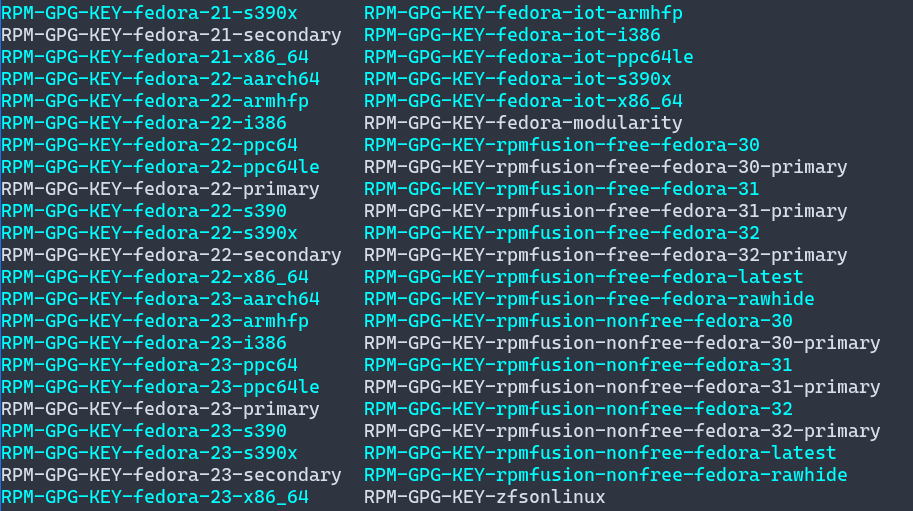
\includegraphics[width=\textwidth,height=0.6\textheight]{Abbildungen/GPG.png}
\end{frame}

\begin{frame}{}
\protect\hypertarget{section}{}
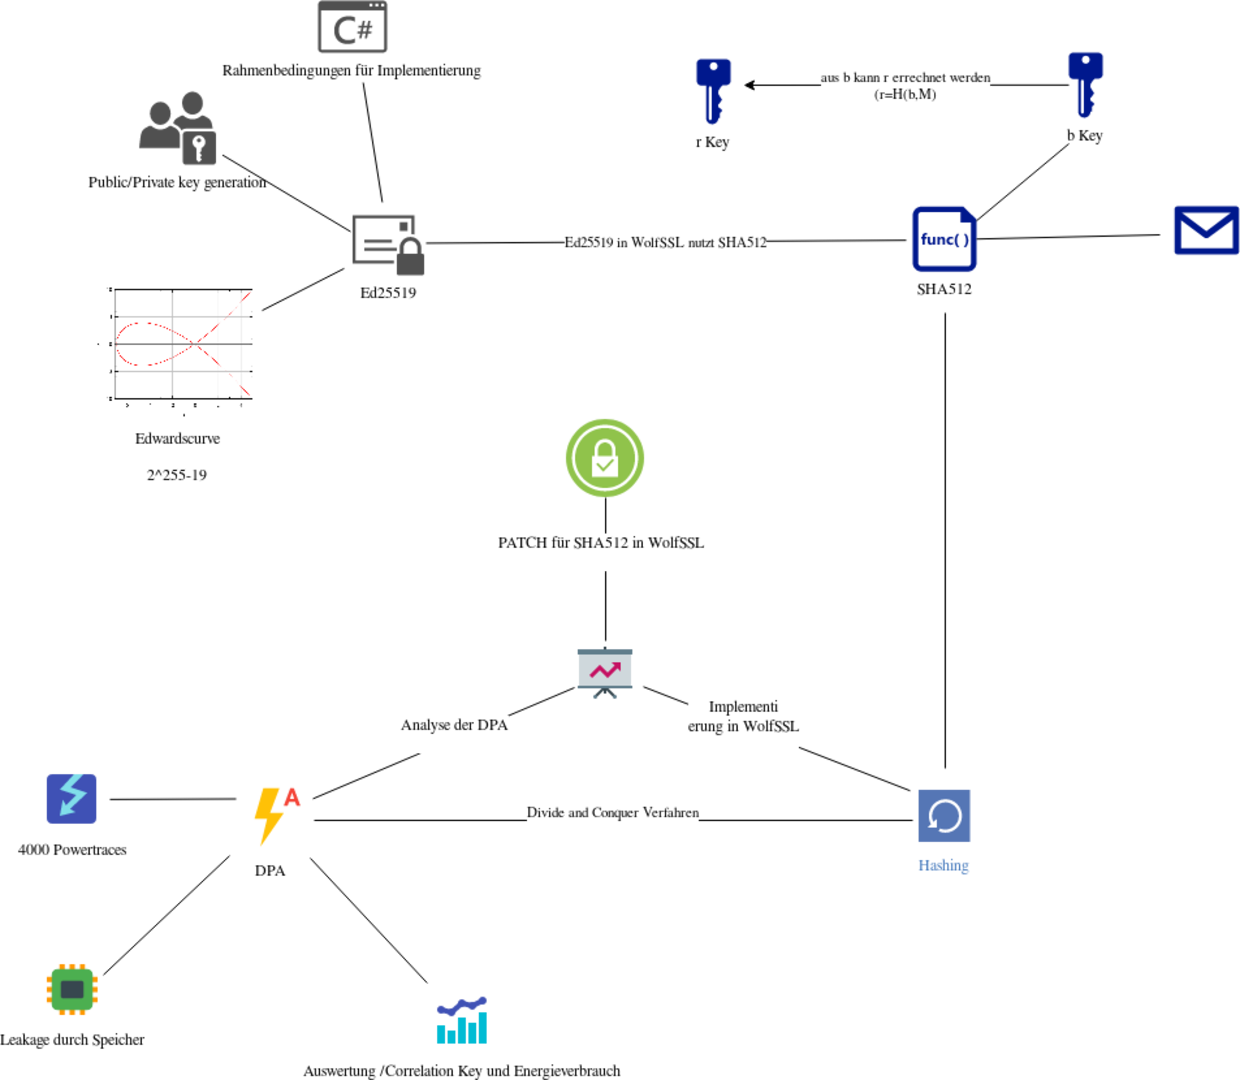
\includegraphics{Abbildungen/ITSEC(1)_res.png}
\end{frame}

\begin{frame}{}
\protect\hypertarget{section-1}{}
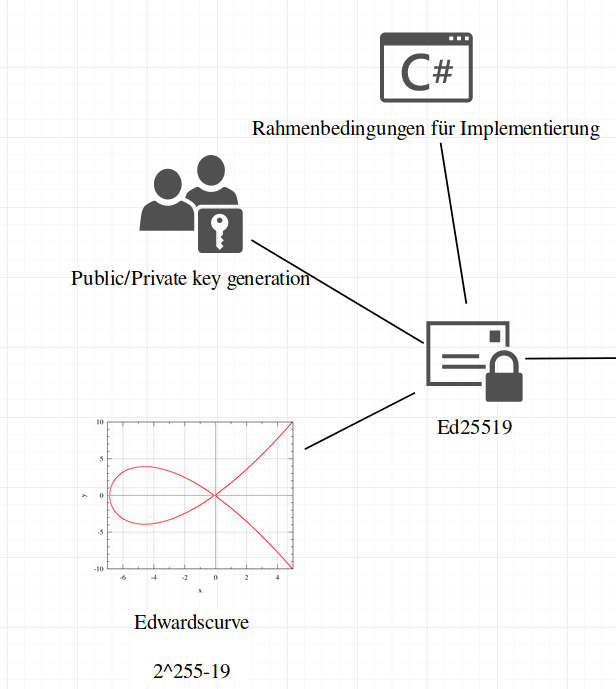
\includegraphics{Abbildungen/Punkt1.png}
\end{frame}

\begin{frame}{EDCSA \& Ed25519}
\protect\hypertarget{edcsa-ed25519}{}
\begin{itemize}
\tightlist
\item
  Signaturverfahren basierend auf Eliptic Curve Cryptography (EEC)

  \begin{itemize}
  \tightlist
  \item
    Basis ist eine Punktruppe einer Elliptischen Kurve
  \end{itemize}
\item
  RSA → Faktosisierungsproblem (Primzahlen)
\item
  ECDSA ist verbereitet

  \begin{itemize}
  \tightlist
  \item
    EdDSA (Edwardscurve)
  \item
    Ed25519 (Edwardscurve 25519)
  \end{itemize}
\item
  160bit EEC Schlüssel = 1200bit RSA Schlüssel

  \begin{itemize}
  \tightlist
  \item
    Speicherverbrauch, Energieverbrauch (IoT)\\
    siehe (Hühnlein and Korte 2006; Susella 2018)
  \end{itemize}
\end{itemize}
\end{frame}

\begin{frame}{EDCSA \& Ed25519}
\protect\hypertarget{edcsa-ed25519-1}{}
\begin{itemize}
\tightlist
\item
  Verwendung (Susella 2018)

  \begin{itemize}
  \tightlist
  \item
    OpenSSH
  \item
    WolfSSL / OpenSSL / LibreSSL / GnuTLS
  \item
    Tor Protokoll
  \item
    DNS Protokolle
  \item
    Signal Messenger Protokoll
  \end{itemize}
\end{itemize}


\includegraphics{Abbildungen/openssh.png}
\end{frame}

\begin{frame}{Ed25519 Funktionsweise}
\protect\hypertarget{ed25519-funktionsweise}{}
\textbf{Tafelbild}
\end{frame}

\begin{frame}{}
\protect\hypertarget{section-2}{}
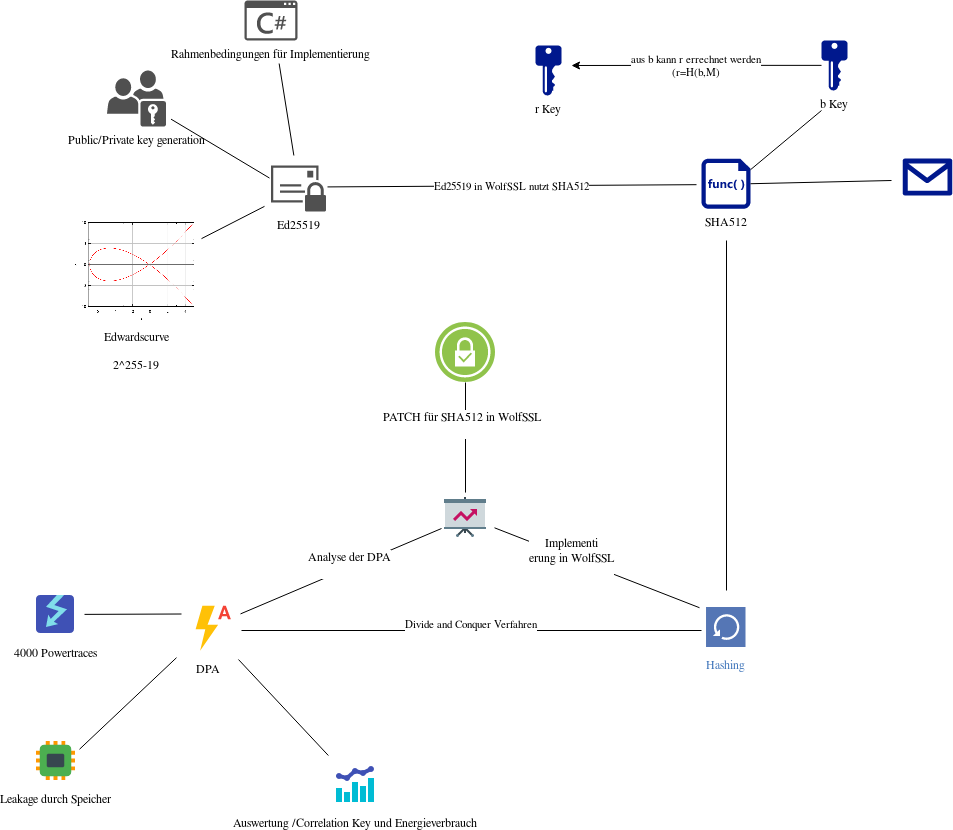
\includegraphics{Abbildungen/ITSEC(1).png}
\end{frame}

\begin{frame}{}
\protect\hypertarget{section-3}{}
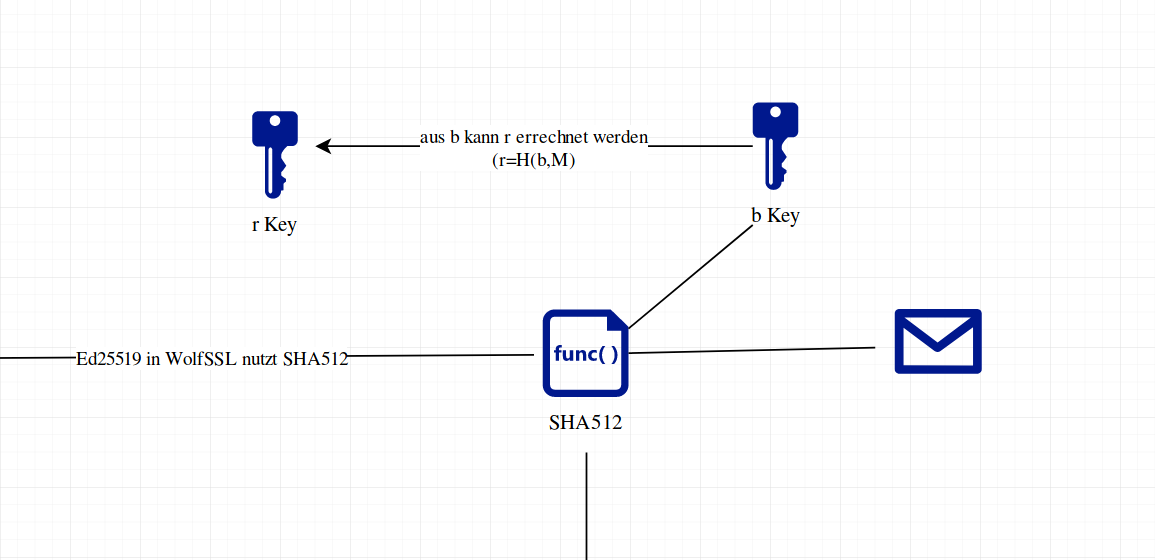
\includegraphics{Abbildungen/Punkt2.png}
\end{frame}

\begin{frame}[fragile]{Secure Hash ``SHA512''}
\protect\hypertarget{secure-hash-sha512}{}
\begin{itemize}
\tightlist
\item
  Ed25519 nutzt SHA512

  \begin{itemize}
  \tightlist
  \item
    Merkle--Damgård Konstruktion

    \begin{itemize}
    \tightlist
    \item
      Erweiterung um Davies-Meyer
    \end{itemize}
  \item
    SHA-2 Familie (SHA256,SHA512) → Bitlänge des Hash
  \end{itemize}
\item
  Auxiliary Schlüssel b
\end{itemize}

\begin{verbatim}
Message M (v. Länge) → SHA512 Funktion → 512 Bit Ausgabe
\end{verbatim}

(Susella 2018)
\end{frame}

\begin{frame}{Secure Hash ``SHA512'' II}
\protect\hypertarget{secure-hash-sha512-ii}{}
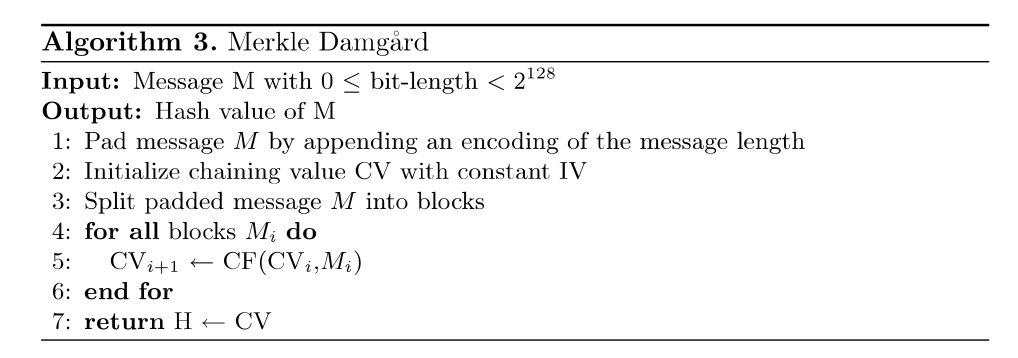
\includegraphics{Abbildungen/MD.png}
\end{frame}

\begin{frame}{Secure Hash ``SHA512'' III}
\protect\hypertarget{secure-hash-sha512-iii}{}
\begin{itemize}
\tightlist
\item
  Ausgabe 512 Bit
\item
  Größe des internen Status 512 Bit
\item
  Blockgröße 1024 Bit

  \begin{itemize}
  \tightlist
  \item
    16 Wörter
  \item
    Wortgröße von 64 Bit
  \end{itemize}
\item
  80 Runden
\item
  Operationen auf Status

  \begin{itemize}
  \tightlist
  \item
    AND / XOR
  \item
    Addition (mod 2\textsuperscript{64}) (Susella 2018)
  \end{itemize}
\end{itemize}
\end{frame}

\begin{frame}{}
\protect\hypertarget{section-4}{}
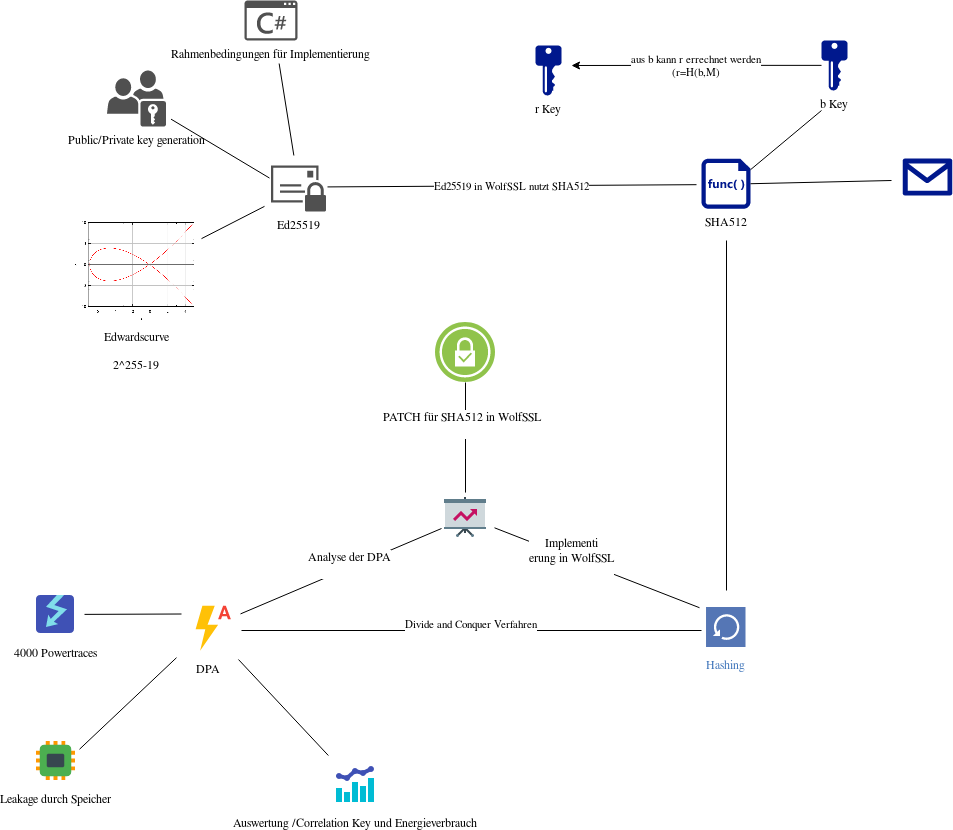
\includegraphics{Abbildungen/ITSEC(1).png}
\end{frame}

\begin{frame}{}
\protect\hypertarget{section-5}{}
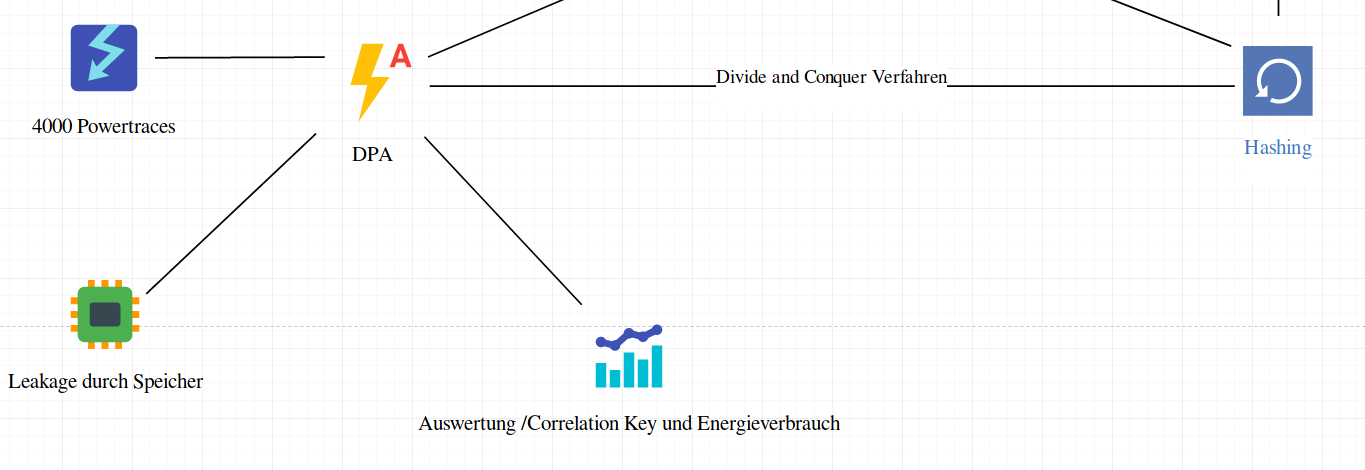
\includegraphics{Abbildungen/Punkt4.png}
\end{frame}

\begin{frame}{Angriff auf Ed25519}
\protect\hypertarget{angriff-auf-ed25519}{}
\begin{itemize}
\tightlist
\item
  \textbf{Key Recovery} Attacke

  \begin{itemize}
  \tightlist
  \item
    Energieverbrauch eines SOCs
  \end{itemize}
\item
  Angriff bei Berechnung der ``flüchtigen'' Schlüssel

  \begin{itemize}
  \tightlist
  \item
    von Interesse ist Schlüssel b
  \end{itemize}
\item
  Hilfsschlüssel r bekannt

  \begin{itemize}
  \tightlist
  \item
    Scalar a, Hilfsschlüssel b → manipulierte Signaturen
  \end{itemize}
\end{itemize}
\end{frame}

\begin{frame}{Angriff auf Ed25519 II}
\protect\hypertarget{angriff-auf-ed25519-ii}{}
\begin{itemize}
\tightlist
\item
  Differential Power Analysis (DPA)

  \begin{itemize}
  \tightlist
  \item
    SDA → Abhängigkeit Daten und Energieverbrauch
  \item
    Energieverbrauch an einem Punkt der Encryption
  \end{itemize}
\item
  Zwischenwert (Interdemediate Value)

  \begin{itemize}
  \tightlist
  \item
    Value mit bekanntem Teil/Message
  \item
    Wert als Funktion darstellbar
  \end{itemize}
\end{itemize}

\[ f(d,k) = Value \]
\end{frame}

\begin{frame}[fragile]{Angriff auf Ed25519 III}
\protect\hypertarget{angriff-auf-ed25519-iii}{}
\begin{itemize}
\tightlist
\item
  64 bit unbekannte Bits

  \begin{itemize}
  \tightlist
  \item
    2\textsuperscript{64} mögliche Schlüssel
  \end{itemize}
\item
  Divide-and-Conquer Strategie

  \begin{itemize}
  \tightlist
  \item
    8 Bit → 256 mögliche Schlüssel
  \end{itemize}
\end{itemize}

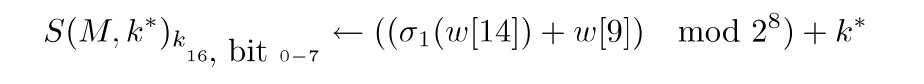
\includegraphics[width=\textwidth,height=0.6\textheight]{Abbildungen/keyDPA.png}

\begin{itemize}
\tightlist
\item
  Hamming Weight wird berechnet (Anzahl Traces X Key Kandidaten)
\item
  Pearson Korrelation der Zeit (Time Samples, Hamming Weight )
\end{itemize}

\begin{verbatim}
Zu jedem Schlüssel Kandidaten muss jedes    
Time sample eines Traces zugeordnet werden    
→ korrekte Ausrichtung für jeden Schlüssel  
→ Vergleichbarkeit
\end{verbatim}
\end{frame}

\begin{frame}{Angriff auf Ed25519 IIII}
\protect\hypertarget{angriff-auf-ed25519-iiii}{}
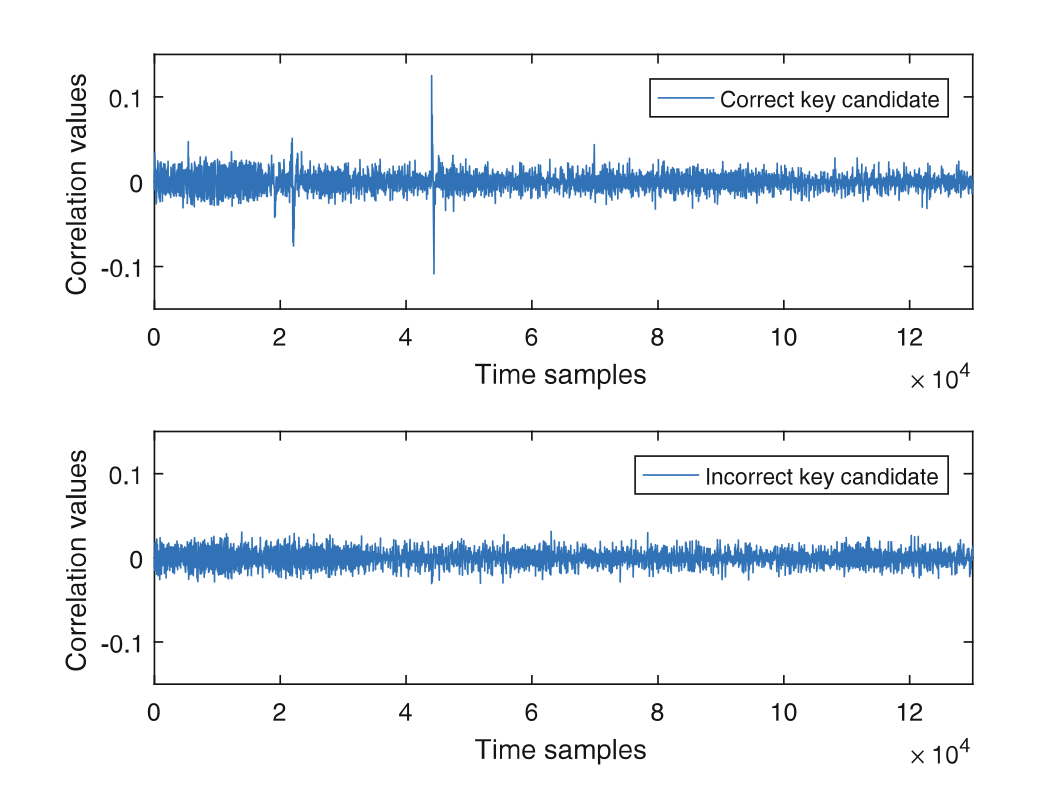
\includegraphics{Abbildungen/cvDPA.png}
\end{frame}

\begin{frame}{}
\protect\hypertarget{section-6}{}
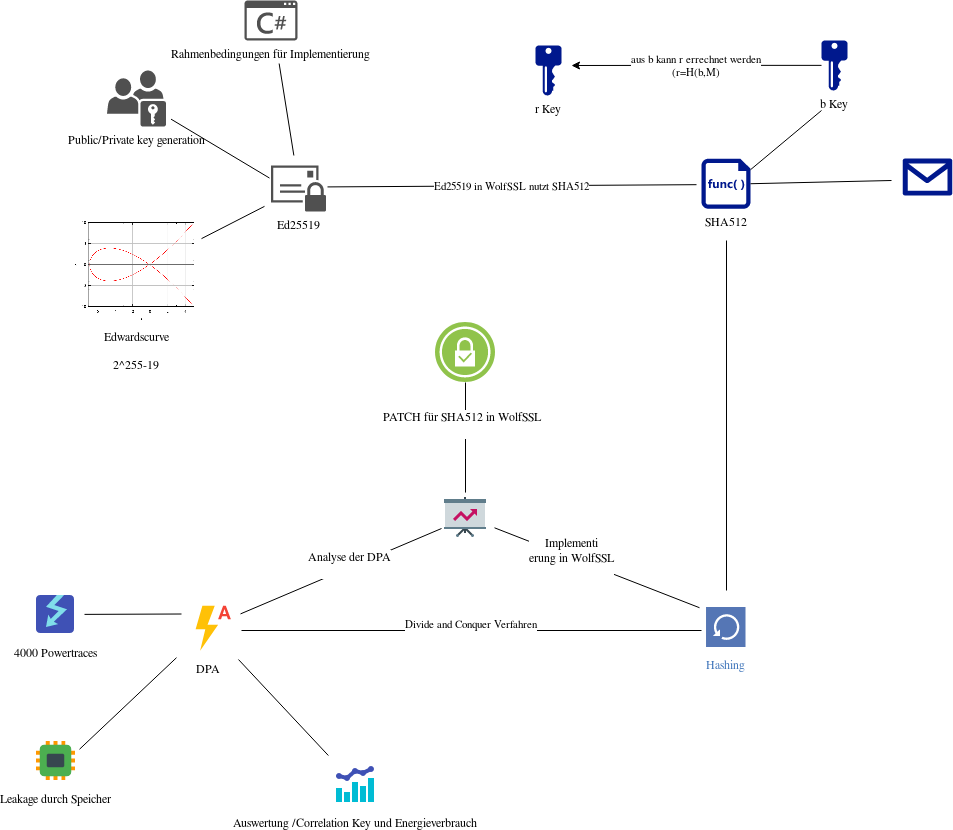
\includegraphics{Abbildungen/ITSEC(1).png}
\end{frame}

\begin{frame}{}
\protect\hypertarget{section-7}{}
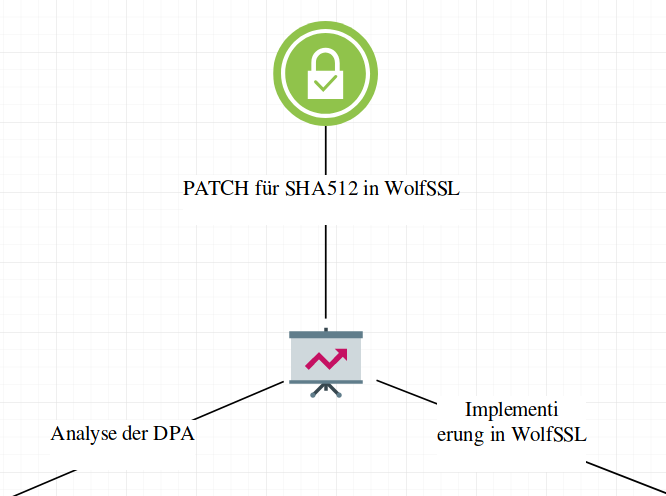
\includegraphics{Abbildungen/Punkt5.png}
\end{frame}

\begin{frame}{Verbesserung \& Gegenmaßnahmen}
\protect\hypertarget{verbesserung-gegenmauxdfnahmen}{}
\begin{itemize}
\item
  Schlüssel \& Nachricht nicht gemeinsam in Kompressionsfunktion
\item
  Padding bereits bei Schlüssel durchführen

  \begin{itemize}
  \tightlist
  \item
    Random Werte
  \end{itemize}
\item
  Vorteil

  \begin{itemize}
  \tightlist
  \item
    Verifikation Sigantur bleibt gleich
  \item
    Implemetierung des SHA wird geändert
  \end{itemize}
\item
  Nachteil für IoT

  \begin{itemize}
  \tightlist
  \item
    Verlust der deterministischen Berechnung
  \item
    Berechnungszeit steigt
  \end{itemize}
\end{itemize}
\end{frame}

\begin{frame}{}
\protect\hypertarget{section-8}{}
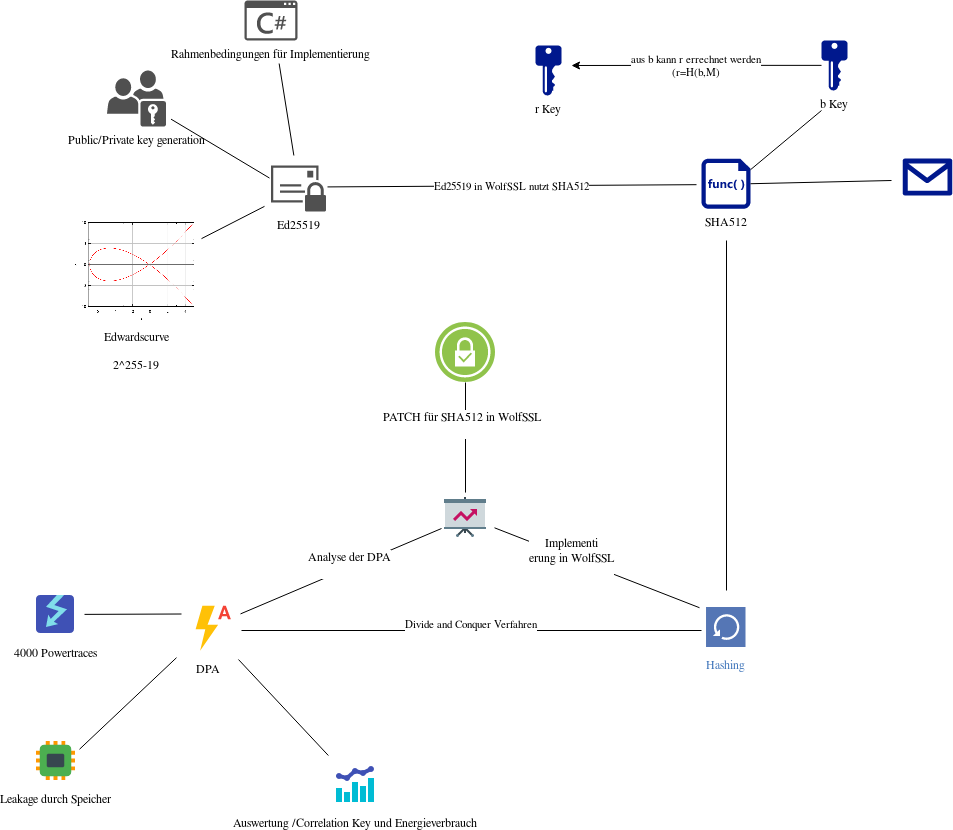
\includegraphics{Abbildungen/ITSEC(1).png}
\end{frame}

\begin{frame}{Literatur}
\protect\hypertarget{literatur}{}
\hypertarget{refs}{}
\begin{cslreferences}
\leavevmode\hypertarget{ref-huhnlein2006grundlagen}{}%
Hühnlein, Detlef, and Ulrike Korte. 2006. \emph{Grundlagen Der
Elektronischen Signatur: Recht-Technik-Anwendung}. SecuMedia-Verlag.

\leavevmode\hypertarget{ref-katz1996handbook}{}%
Katz, Jonathan, Alfred J Menezes, Paul C Van Oorschot, and Scott A
Vanstone. 1996. \emph{Handbook of Applied Cryptography}. CRC press.

\leavevmode\hypertarget{ref-susella2018breaking}{}%
Susella, Ruggero. 2018. ``Breaking Ed25519 in Wolfssl.'' In \emph{Topics
in Cryptology--Ct-Rsa 2018: The Cryptographers' Track at the Rsa
Conference 2018, San Francisco, ca, Usa, April 16-20, 2018,
Proceedings}, 10808:1. Springer.
\end{cslreferences}
\end{frame}

\end{document}
